\subsection{Normalized Angular Velocity Input}

We have the no-load dynamic model for the BLDC motor with propeller:
\begin{align*}
    J \dot \omega + b_m \omega + C_D \omega^2+ M_f &= u K_r V_{in}
\end{align*}
At steady state ($\dot \omega = 0$), the above equation becomes:
\begin{align*}
    b_m \omega + C_D \omega^2 +  M_f &= u K_r V_{in}\\
    \implies \frac{b_m}{K_r} \left(\frac{\omega_m}{V_{in}}\right) + \frac{V_{in}}{K_r} C_D \lr{\frac{\omega}{V_{in}}}^2 + \frac{M_f}{K_r V_{in}} &= u
\end{align*}

\itbf{Definition}: Let, $u_{\omega}$ be the angular velocity of the motor with propeller at unit supply voltage for the given pwm input ($u_p$). Also, let us call it "\itbf{Normalized angular velocity}".
\begin{align*}
    u_{\omega} &= \frac{\omega}{V_{in}} \text{  at  } u = g_u(u_p)\\
    \implies u &= \underbrace{\frac{b_m}{K_r} u_\omega + \frac{\hat V_{in}}{K_r} C_D u_\omega^2 + \frac{M_f}{K_r  \hat V_{in}}}_{g_\omega (u_\omega, \hat V_{in})}
\end{align*}

The relationship between $u_\omega$ and $u_p$ can be estimated from the staic measuremnt data.
\begin{figure}[H]
    \begin{minipage}{0.49\textwidth}
    We have:
        \begin{align*}
            u_\omega &= a u_p + b
            \qquad a = 0.0696
            \qquad b = -64.3266\\
        \end{align*}
    Also,
        \begin{align*}
            \because u &= g_\omega(u_\omega, \hat V_{in})\\
            \implies g_u(u_p) &= g_\omega(a u_p  + b, \hat V_{in})\\
        \end{align*}
    \end{minipage}
    \begin{minipage}{0.49\textwidth}
       \begin{figure}[H]
            \centering
            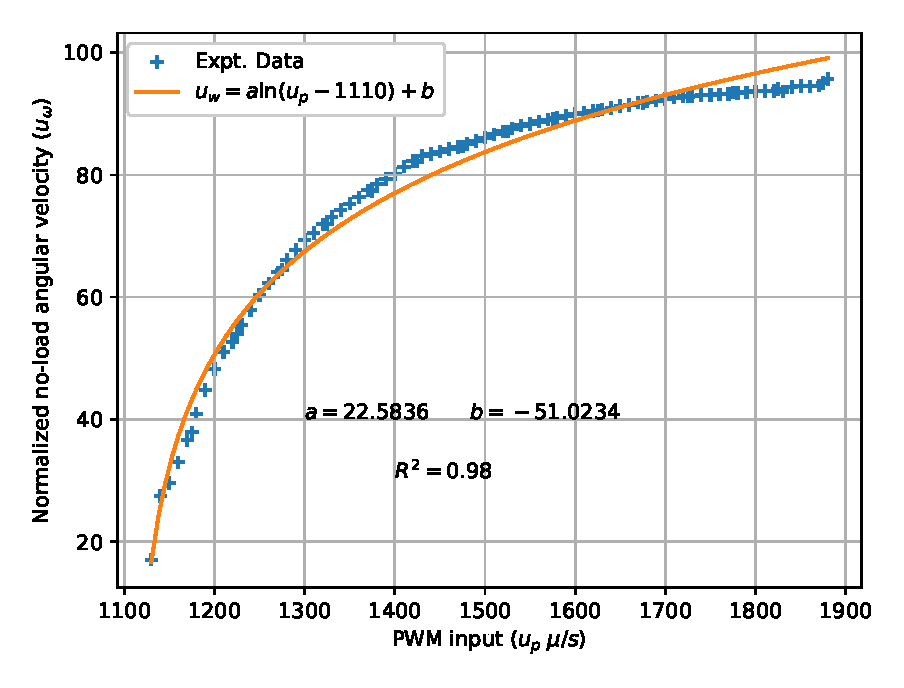
\includegraphics[width = \textwidth]{./figs/norm_omega/no-load_rpm.eps}
            \caption{$u_\omega$ as a function of $u_p$}
        \end{figure}
    \end{minipage}
\end{figure}
